%20 min preso!
\documentclass[xcolor=table]{beamer}
\usepackage{beamerthemesplit}
\usepackage{wrapfig}
\usetheme{SPbGU}
\usepackage{pdfpages}
\usepackage{amsmath}
\usepackage{cmap}
\usepackage[T2A]{fontenc}
\usepackage[utf8]{inputenc}
\usepackage[english]{babel}
\usepackage{indentfirst}
\usepackage{amsmath}
\usepackage{tikz}
\usepackage{multirow}
\usepackage[noend]{algpseudocode}
\usepackage{algorithm}
\usepackage{algorithmicx}
\usepackage{fancyvrb}
\usetikzlibrary{calc}
\usetikzlibrary{shapes,arrows}
\usetikzlibrary{arrows,automata}
\usetikzlibrary{positioning}

\usepackage{tabularx}
\newcolumntype{Y}{>{\raggedleft\arraybackslash}X}

\renewcommand{\thealgorithm}{}

\newtheorem{mytheorem}{Theorem}
\renewcommand{\thealgorithm}{}

\newcommand{\tikzmark}[1]{\tikz[overlay,remember picture] \node (#1) {};}
\def\Put(#1,#2)#3{\leavevmode\makebox(0,0){\put(#1,#2){#3}}}

\newcommand{\ltz}{$< 1$}


\tikzset{
    state/.style={
           rectangle,
           rounded corners,
           draw=black, very thick,
           minimum height=2em,
           inner sep=2pt,
           text centered,
           },
}

\beamertemplatenavigationsymbolsempty

\title[Parsing for String-Searching Problem]{Modification of Valiant's Parsing Algorithm for String-Searching Problem}
%\subtitle[YaccConstructor]{Parsing techniques for graph analysis}
% То, что в квадратных скобках, отображается в левом нижнем углу.
\institute[JetBrains Research]{
JetBrains Research, Programming Languages and Tools Lab  \\
Saint Petersburg University
}

% То, что в квадратных скобках, отображается в левом нижнем углу.
\author[Yuliya Susanina]{Semyon Grigorev, \textbf{Yuliya Susanina}, Anna Yaveyn}

\date{September 6, 2019}

\begin{document}
{
\begin{frame}[fragile]
  \begin{table}
  \centering
  \begin{tabularx}{\linewidth}{YcX}
    
\includegraphics[height=1.5cm]{pic/jetbrainsResearch.pdf} \hfill
    & \begin{minipage}[t]{0.3\textwidth}\center \vspace{-1cm} CIBB 2019
      \end{minipage}
    & \hfill 
\includegraphics[height=1.5cm]{pic/SPbGU_Logo.png}
  \end{tabularx}
  \end{table}
  \titlepage
\end{frame}
}

\begin{frame}[fragile] \frametitle{Formal grammars and languages}

    \begin{itemize}
      \item $G = (\Sigma, N, R, S)$ --- context-free grammar (CFG) in normal Chomsky form
      \begin{itemize}
        \item $A \rightarrow B C$, where $A, B, C \in N$
        \item $A \rightarrow a$, where $A \in N, a \in \Sigma$
        \item $S \rightarrow \varepsilon$, where $\varepsilon$ is an empty string
      \end{itemize}
      \item $L_G (A) = \{ \omega \mid A \Rightarrow^* \omega \}$, where $A \in N$, $\omega \in \Sigma^*$
      \item Parsing --- does $\omega$ belong to $ L_G (S)$?
    \end{itemize}

\end{frame}

\begin{frame}[fragile] \frametitle{RNA analysis}

\begin{itemize}
    \item RNA sequences are treated as strings over $\{A, G, C, U\}$
    \item Formal grammars describe RNA secondary structure features
    \item Parsing as method to find all strings or substrings with these features
    \item Applications: RNA secondary structure prediction, classification and recognition problems
    \begin{itemize}
        \item \emph{Eddy S. R., Durbin R.} "RNA Sequence Analysis Using Covariance Models" 1994
        \item \emph{Knudsen B., Hein J.} “Rna secondary structure prediction using stochastic context-free grammars and evolutionary history” 1999
        \item \emph{Grigorev S., Lunina P.} “The composition of dense neural networks and formal grammars for secondary structure analysis” 2019
    \end{itemize}
\end{itemize}
    
\end{frame}



%\begin{frame}[fragile] \frametitle{CFG-based approaches: expressiveness}
%    \begin{itemize}
%        \item Conjunctive grammars \\
%         \small{(+)} $A \rightarrow B_1 C_1\& \ldots \&B_m C_m$
%        \item Boolean grammars \\
%         \small{(+)} $A \rightarrow B_1 C_1\& \ldots \&B_m C_m \& \neg D_1 E_1~\& \ldots \& \neg D_n E_n$
%\end{itemize}
%\end{frame}

\begin{frame}[fragile] \frametitle{Tabular parsing algorithms}

\begin{itemize}
    \item Input:
    \begin{itemize}
        \item Grammar $G = (\Sigma, N, R, S)$ in Chomsky normal form
        \item String $\omega = a_{1}a_{2} \dots a_{n}$, $a_i \in \Sigma$
    \end{itemize}
    \item Parsing table $T$:
        \begin{itemize}
            \item $T_{i, j} =  \{ A | A \in N, a_{i + 1} \dots a_{j} \in L_{G}(A)\} \quad \forall i < j$
            \item $\omega \in L_{G}(S) \iff S \in T_{0, n}$
        \end{itemize}
    \item Process of filling:
        \begin{itemize}
            \item $T_{i - 1, i} = \{ A | A \rightarrow a_{i} \in R\}$
            \vspace{5}
            \item $T_{i, j} = f(P_{i, j})$, where $P_{i, j} = \bigcup\limits_{k = i + 1}^{j - 1} T_{i,k} \times T_{k, j}$ \\ 
            \hspace{85} $f(P_{i, j}) = \{A | \exists A \rightarrow BC \in R : (B, C) \in P_{i, j}\}$
        \end{itemize}
    
\end{itemize}
\end{frame}



\begin{frame}[fragile] \frametitle{Computational complexity}
    
    \begin{itemize}
        \item CYK: $\mathcal{O}(|G|n^3)$  \\
        \emph{Younger, D. H.} "Context-free language processing in time $n^3$" 1966
        \item GFPQ: $\mathcal{O}(|G|n^2BMM(n))$ \\
        \emph{Azimov, R. and Grigorev, S.}  "Context-free path querying by matrix multiplication" 2018
        \vspace{5}
        \pause
        \item Valiant: $\mathcal{O}(|G|BMM(n)log(n))$ \\
        \emph{Valiant, L. G.} "General context-free recognition in less than cubic time" 1975
    \end{itemize}
    
  
    \onslide<2>{\tikz[overlay,remember picture]{\draw[draw=red,thick,double,fill opacity=0.2] ($(0.2,0.4)$) rectangle ($ (12,2.1)$);}}
    
\end{frame}

\begin{frame}[fragile] \frametitle{Valiant's parsing algorithm}

\begin{itemize}
    \item Reduction to matrix multiplication \\ \vspace{4}
    $X, Y \in T$ \\
    $X \times Y = Z$, where $Z_{i, j} = \bigcup\limits_{k = 1}^{l} X_{i, k} \times Y_{k, j}$
    
    \item Reduction to Boolean matrix multiplication \\ \vspace{4}
    $Z_{i, j}^{(B, C)} = 1 \iff (B, C) \in Z_{i, j}$ \\ \vspace{2}
    $Z^{(B, C)} = X^{B} \times Y^{C}$
    
\end{itemize}

\end{frame}


\begin{frame}[fragile] \frametitle{Layered submatrices processing (1)}

    \vspace{55}
    \begin{itemize}
    \item Rearranging the order in which \linebreak submatrices are processed in \linebreak Valiant's algorithm
    \item Division the parsing table into \linebreak layers of disjoint submatrices
    \end{itemize}
        
    \begin{overprint}
        \onslide<1>\vspace{-130}\hspace{165}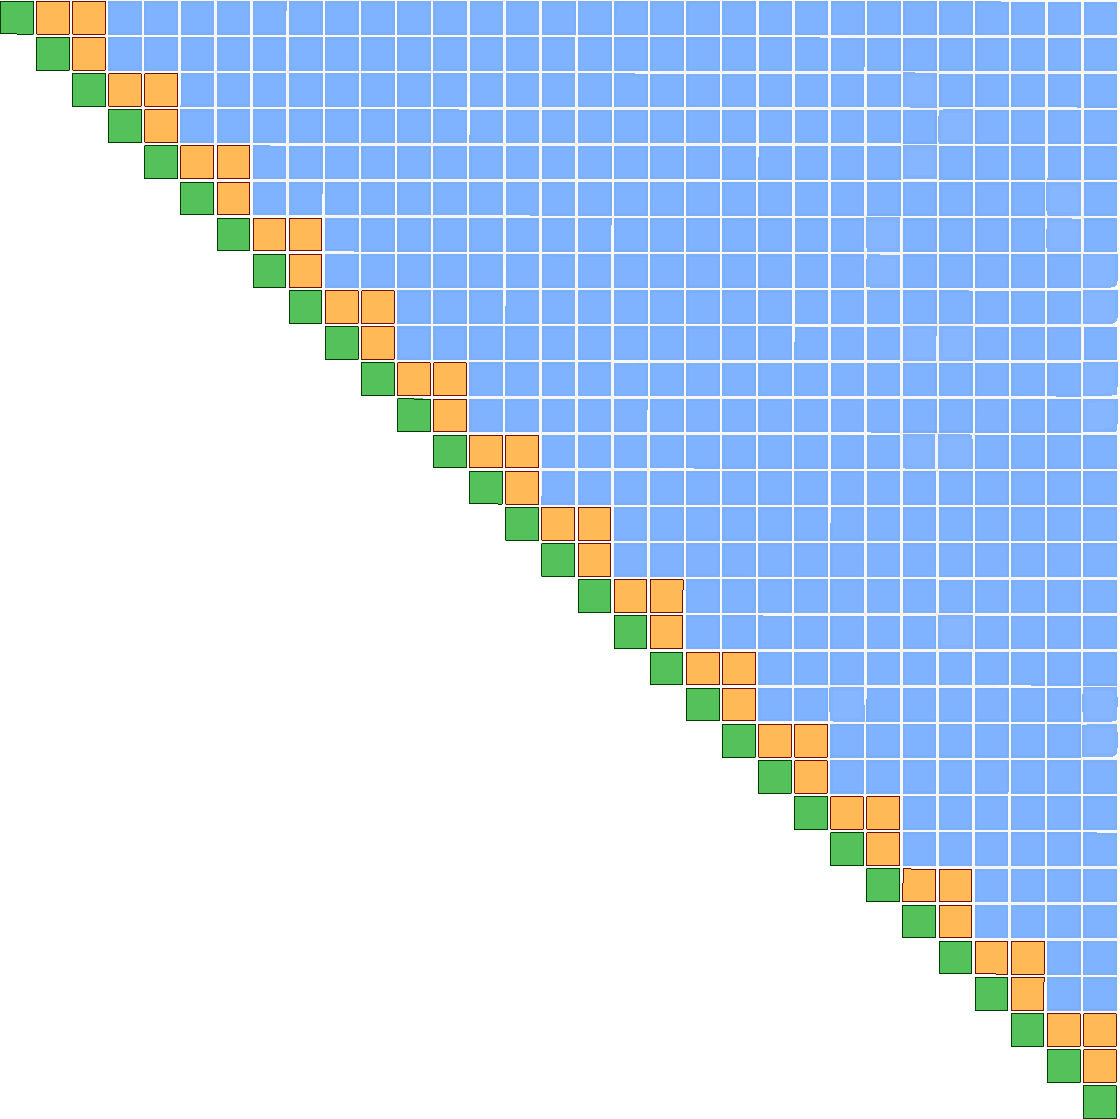
\includegraphics[width = 0.5\linewidth, right]{pic/01.pdf}
        \onslide<2>\vspace{-130}\hspace{165}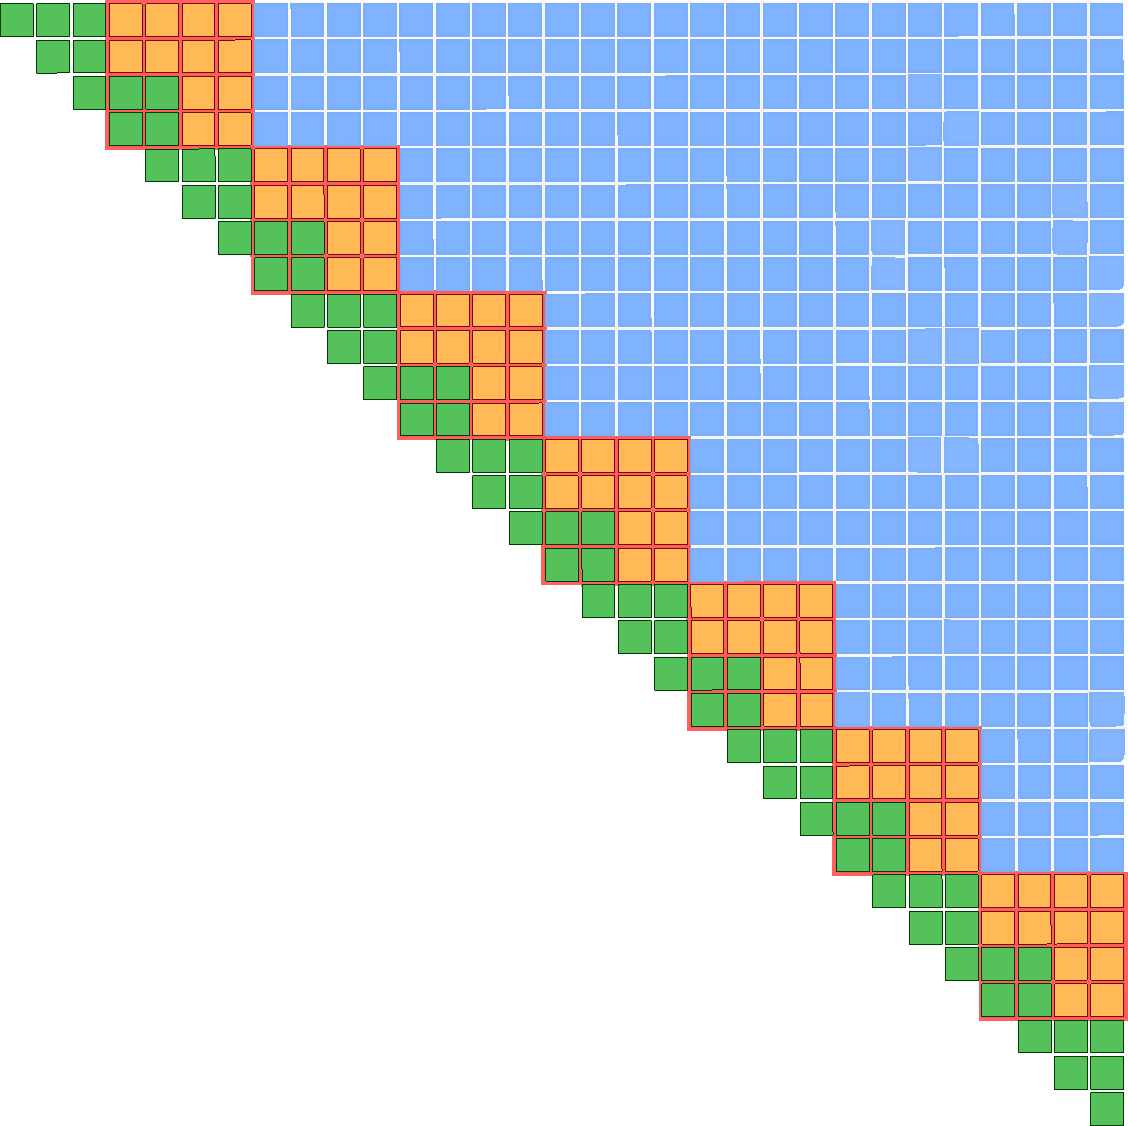
\includegraphics[width = 0.5\linewidth, right]{pic/02.pdf}
        \onslide<3>\vspace{-130}\hspace{165}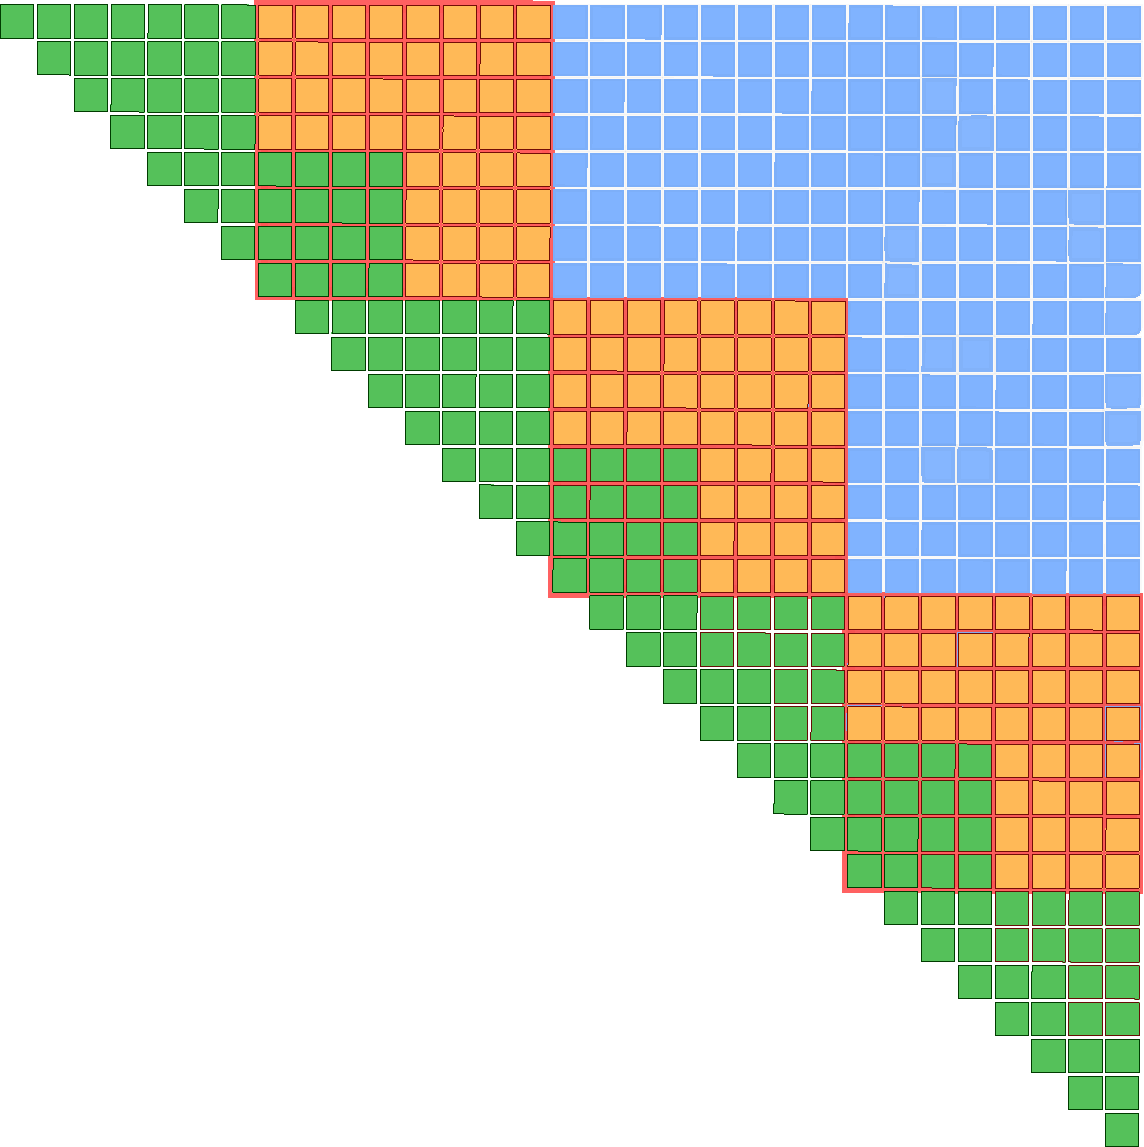
\includegraphics[width = 0.5\linewidth, right]{pic/03.pdf}
        \onslide<4>\vspace{-130}\hspace{165}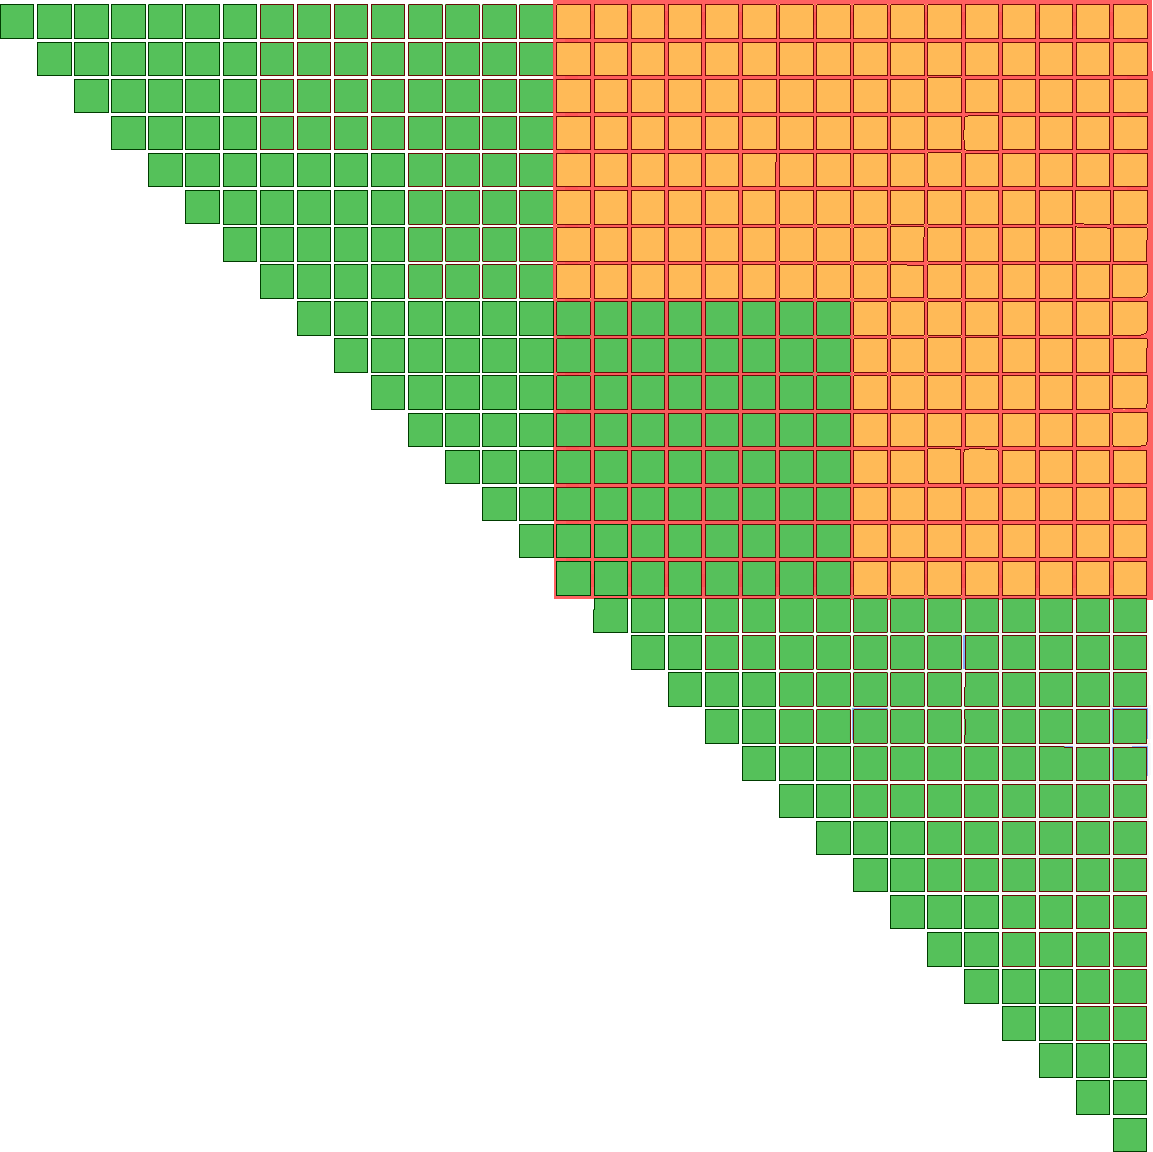
\includegraphics[width = 0.5\linewidth, right]{pic/04.pdf}
        \onslide<5>\vspace{-130}\hspace{165}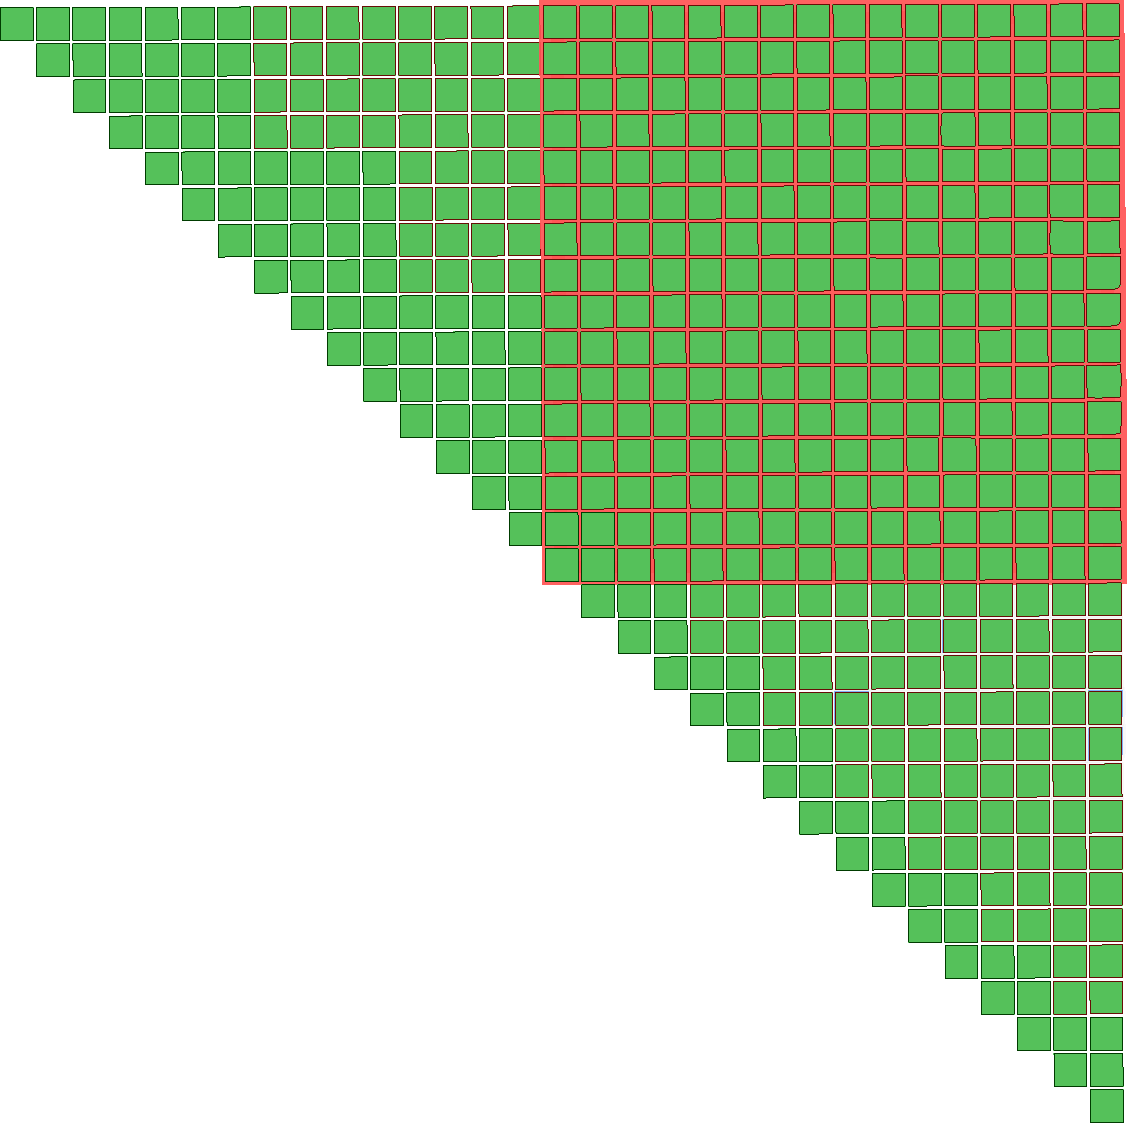
\includegraphics[width = 0.5\linewidth, right]{pic/05.pdf}
    \end{overprint}
    
\end{frame}

\begin{frame}[fragile] \frametitle{Layered submatrices processing (2)}

    \begin{itemize}
    \item Each matrix in the layer can be handled independently
    \item Increasing the lever of parallelism: 
    \begin{itemize}
        \item Matrix multiplication 
        \item Each matrix in layer
        \item Each pair of nonterminals
    \end{itemize}
    \end{itemize}

        \begin{center}
        %\vskip5pt
        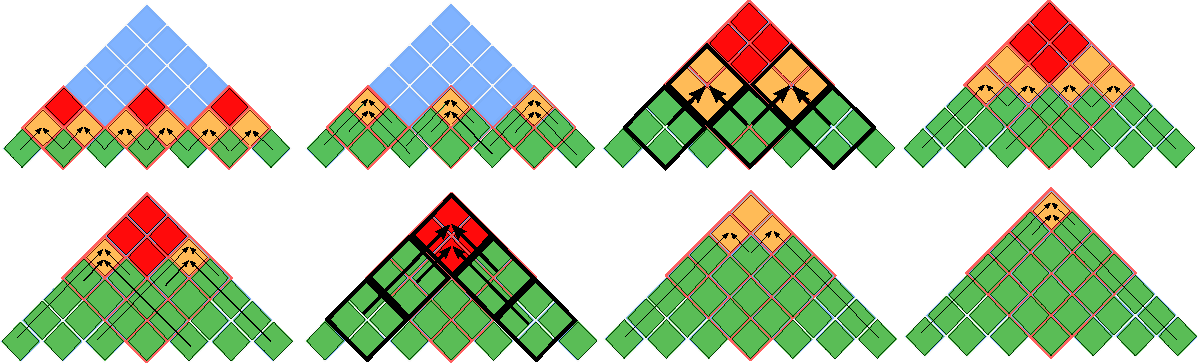
\includegraphics[width=.90\textwidth]{pic/modivis_again.pdf} 
        \end{center} 
    
\end{frame}

\begin{frame}[fragile] \frametitle{String-searching problem}

    \begin{itemize}
      \item \textbf{Problem:} for input string of length $n = 2^p - 1$ find all substrings of length \textit{s} which belong to $L_G(S)$
      \item \textbf{Valiant's algorithm:} it is necessary to calculate at least 2 triangle submatrices of size $\frac{n}{2}$ \\ 
      $\mathcal{O}(|G|BMM(2^{p - 1})(p - 2))$
  \end{itemize}

    \begin{overprint}
        \onslide<1>\centering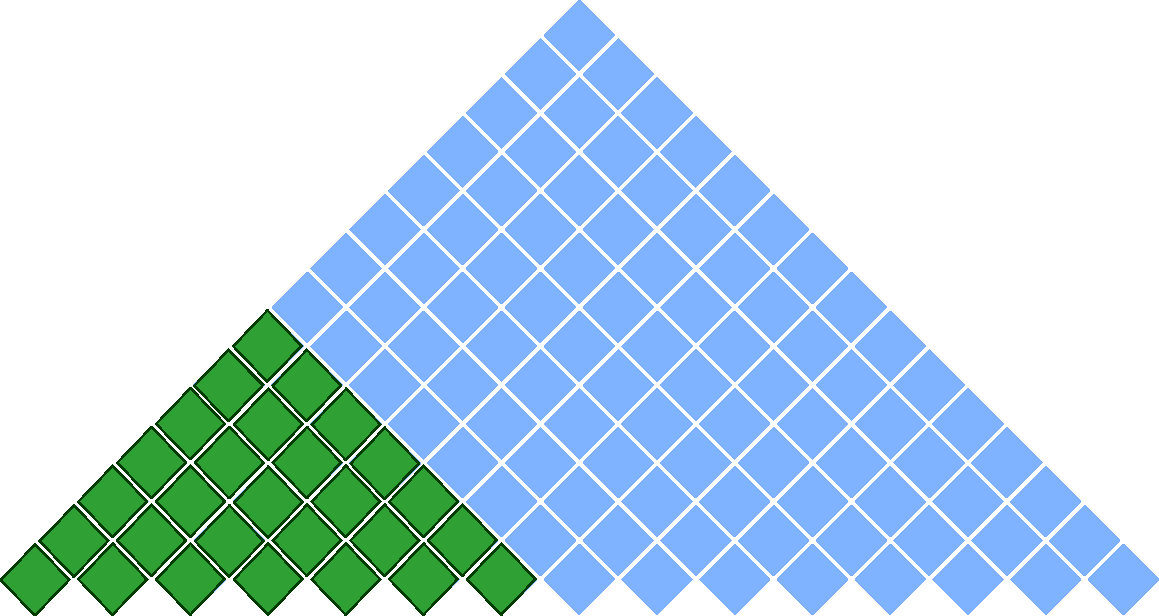
\includegraphics[width = 0.5\linewidth]{pic/valsubstring1.pdf}
        \onslide<2>\centering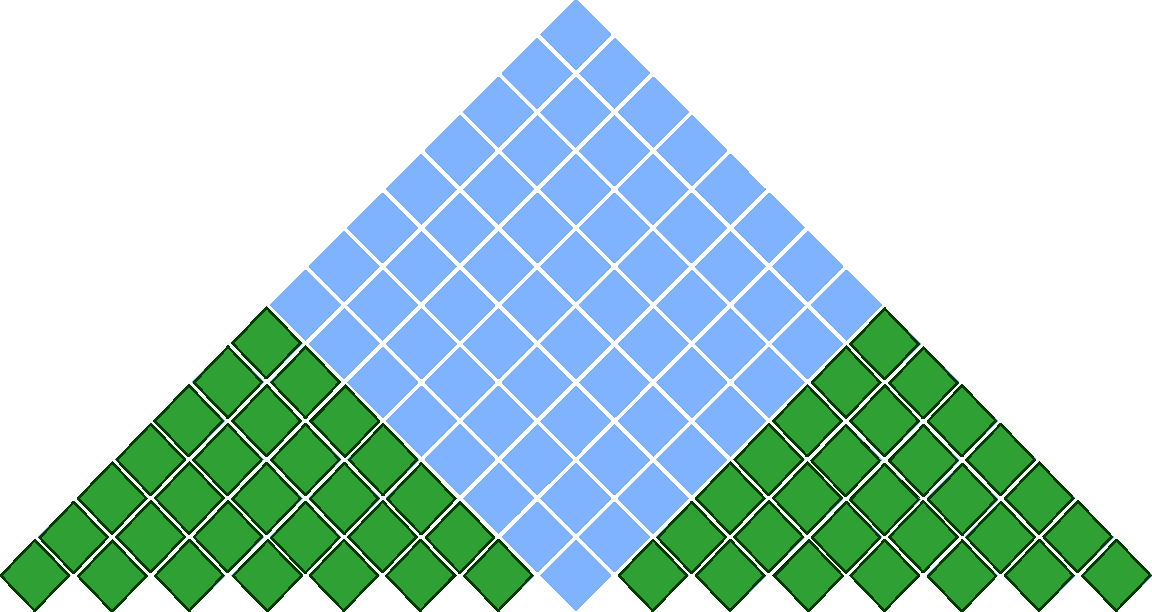
\includegraphics[width = 0.5\linewidth]{pic/valsubstring2.pdf}
        \onslide<3>\centering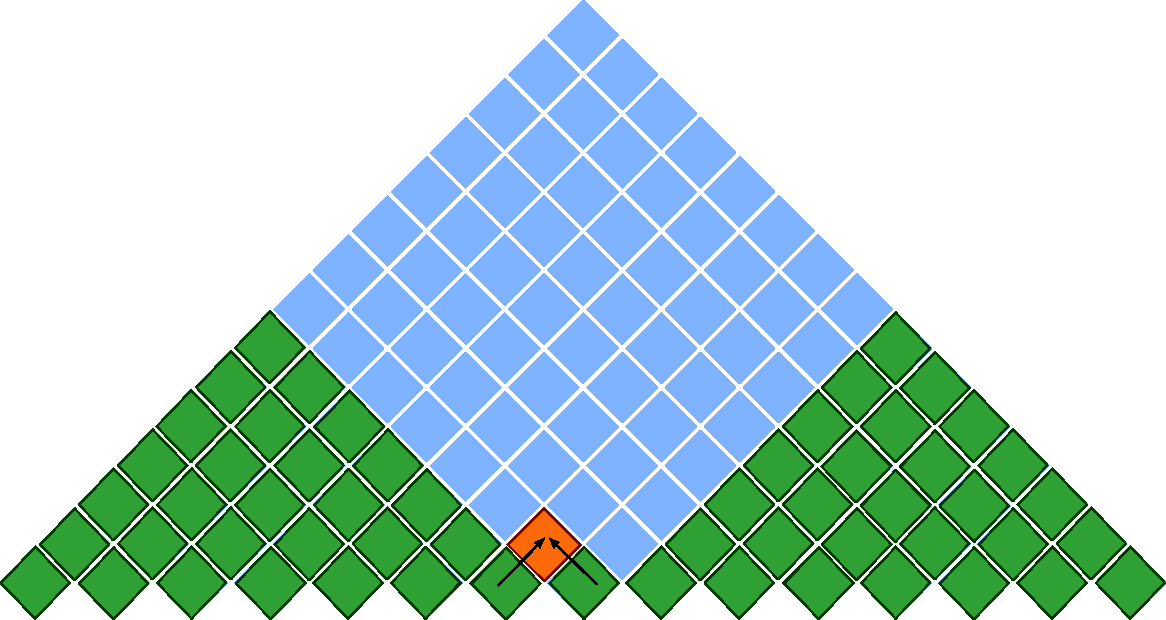
\includegraphics[width = 0.5\linewidth]{pic/valsubstring3.pdf}
        \onslide<4>\centering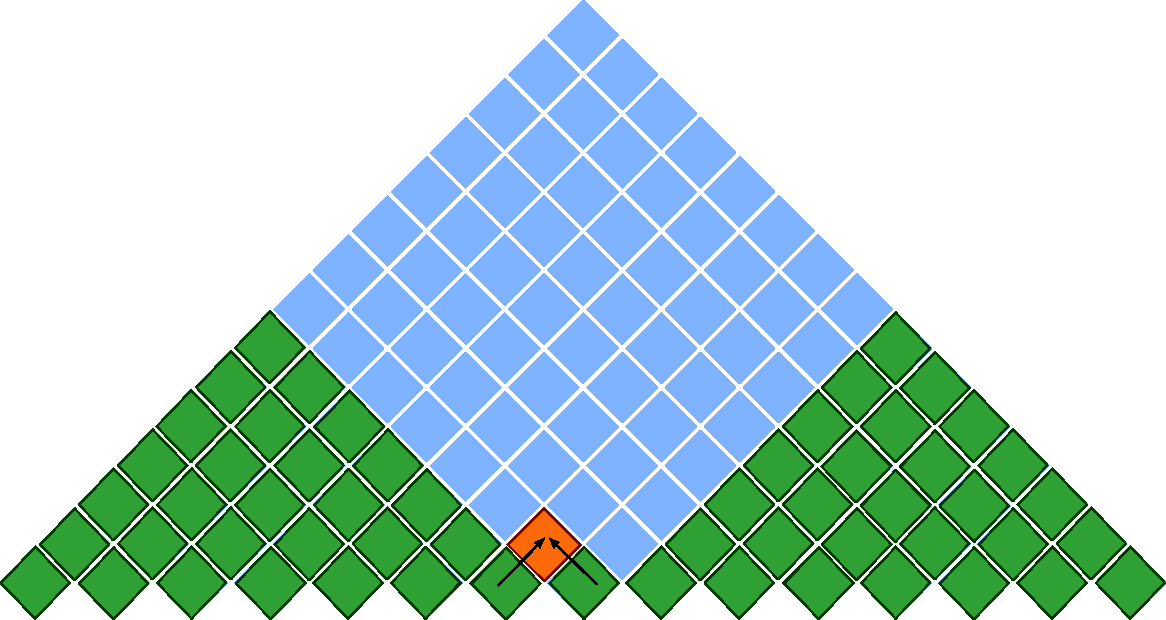
\includegraphics[width = 0.5\linewidth]{pic/valsubstring3.pdf}
    \end{overprint}

    \pause
    \onslide<4>
    \begin{itemize}
      \item  \textbf{Modification:} it is necessary to compute layers with submatrices of size not greater than $2^r$, где $2^{r-2} < s \le 2^{r - 1}$ \\
      $\mathcal{O}(|G|2^{2(p - r) - 1}BMM(2^{r})(r - 1))$
  \end{itemize}

\end{frame}

\begin{frame}[fragile] \frametitle{Conclusion}
    \begin{itemize}
        \item We present a modification of Valiant's algorithm 
        \begin{itemize}
            \item Layered submatrices processing
            \item Effective utilization of parallel techniques and GPGPU
            \item Applicability to the string-searching problem
        \end{itemize}
        \item Future research
        \begin{itemize}
            \item High-performance implementation (GPGPU, parallel techniques)
            \item Evaluation on real-world data
            \item Extension for more expressive classes of formal languages \\ (conjunctive,  boolean)
        \end{itemize}
    \end{itemize}
\end{frame}


\begin{frame}
\frametitle{Contact Information}
\begin{itemize}
  \item Yuliya Susanina: \href{mailto:jsusanina@gmail.com}{jsusanina@gmail.com}
  \item Anna Yaveyn: \href{mailto:anya.ayveyn@yandex.ru}{anya.ayveyn@yandex.ru}
  \item Semyon Grigorev: \href{mailto:semen.grigorev@jetbrains.com}{semen.grigorev@jetbrains.com}
\end{itemize}
\vspace{0.1cm}
\center{\huge{Thanks!}}
\end{frame}
\end{document}
